% This is LLNCS.DEM the demonstration file of
% the LaTeX macro package from Springer-Verlag
\documentclass[a4paper,12pt]{llncs}
%
\usepackage{makeidx}  % allows for indexgeneration
\makeindex

\usepackage[ngerman]{babel}
\usepackage[utf8]{inputenc}      % Code-Page latin 1
\usepackage[T1]{fontenc}
% Nur eine der beiden folgenden Zeilen einbinden!
% siehe Abschnitt Bilder
%\usepackage{graphicx}       % Bilder einbinden, Version fuer normales latex
\usepackage[pdftex]{graphicx}       % Bilder einbinden, Version fuer pdflatex

% mit Hyperrefs
\usepackage[pdftex, plainpages=false,hypertexnames=true,pdfnewwindow=true,backref=true,colorlinks=true,citecolor=blue,linkcolor=black,urlcolor=blue,filecolor=blue]{hyperref}% 
% weitere Packages
\usepackage{ifthen}                 % Zum Auskommentieren von Textteilen
\usepackage{amssymb}                % Mathematische Buchstaben
\usepackage{amsmath}                % Verbesserter Formelsatz
\usepackage[vlined,boxed]{algorithm2e}
\usepackage{booktabs}               % schönere Tabellen
\usepackage{color}
\usepackage{hyperref}
 \hypersetup{urlcolor=black,citecolor=black}
%\setalcapskip{1.5ex} % fuer package algorithm
\usepackage{dsfont}  
%\newtheorem{definition}{Definition}
\usepackage{doc}
\usepackage{listings}
\usepackage{subcaption}
\usepackage{url}

% Seitenformat ===============================================================
\hoffset=-1.25truecm
\setlength{\topmargin}{0.0cm}
\setlength{\textheight}{23.0cm}
\setlength{\footskip}{1.5cm}
\setlength{\textwidth}{15.4cm}
\setlength{\evensidemargin}{1.5cm}
\setlength{\oddsidemargin}{1.5cm}
\setlength{\parskip}{1ex}
\setlength{\parindent}{0pt}
\setlength{\marginparwidth}{1.4cm}
\setlength{\marginparsep}{1mm}
\setalcapskip{1.5ex} % fuer package algorithm

\pagestyle{plain}

% Makro-Definitionen ==========================================================
% Zahlenbereiche -------------------------------------------------------------
\newcommand{\N}{{\mathbb{N}}}
\newcommand{\R}{{\mathbb{R}}}
\newcommand{\C}{{\mathbb{C}}}
\newcommand{\Z}{{\mathbb{Z}}}
\newcommand{\Q}{{\mathbb{Q}}}

% 
\def\myverzeichnis{.}

\numberwithin{equation}{section} 
% Bild -----------------------------------------------------------------------
% #1 Filename;  #2 Label;  #3 Bildunterschrift;  #4 Kurzform
\newcommand{\bild}[4]{
  \begin{figure}[htbp]
    \begin{center}
      \includegraphics{#1}
      \caption[#4]{#3}
      \label{#2}
    \end{center}
  \end{figure}
}

% Bildbreite -----------------------------------------------------------------
% #1 Filename;  #2 Breite;  #3 Label;  #4 Bildunterschrift;  #5 Kurzform
\newcommand{\bildbreite}[5]{
  \begin{figure}[htbp]
    \begin{center}
      \includegraphics[width=#2]{#1}
      \caption[#5]{#4}
      \label{#3}
    \end{center}
  \end{figure}
}

% !TeX spellcheck = de_DE
% ============================================================================
\begin{document}

% =========== Das war der Vorspann, jetzt geht's los! ========================

% ============================================================================
% =============  AB HIER DARF UND SOLL GETIPPT WERDEN ========================
% ============================================================================

\author{Yaroslav Nalivayko}
\index{Yaroslav Nalivayko}

% Das Institut wird fuer den Betreuer missbraucht ...
\institute{{\bf Betreuer:} M.Sc. Benjamin Maier}
\authorrunning{Yaroslav Nalivayko}
\title{Newton Fraktale}

\maketitle

\thispagestyle{empty}

\begin{abstract}
Newton Fraktale sind eine Teilmenge der mathematischen Fraktale, die durch Benutzung des Newton Verfahrens für Lösung von nichtlinearen Gleichungen auf Komplexe Ebene erscheinen.
\end{abstract}

% Einleitung -----------------------------------------------------------------
\section{Einleitung}
Newton Fraktale stellen eine interessante Klasse der mathematischen Fraktalen dar. 
Im Rahmen dieser Arbeit werden \nameref{sec:theo} vorgestellt und ein Programm für die \nameref{sec:vis} der Fraktalen entwickelt. In letzte Sektion findet \nameref{sec:analy} mancher interessanten Funktionen statt.


\section{Theoretische Grundlagen}\label{sec:theo}
%Hier werden Grundbegriffe erläutert.
\subsection{Numerische Mathematik}
Die numerische Mathematik beschäftigt sich als Teilgebiet der Mathematik mit der Konstruktion und Analyse von Algorithmen für kontinuierliche mathematische Probleme. \cite{nummath}
Oft wird benutzt, um approximative Lösungen mit Hilfe von Computer zu finden.
\subsection{Newton Verfahren}
Newton Verfahren ist das iterative numerische Verfahren, das eine Wurzel gegebener Funktion findet.	Die Methode ist nach Sir Isaac Newton benannt. \\
Wir interessieren uns in stetig differenzierbaren Funktionen mit nur eine Variable.
\[
f(x) = 0
\] 
Man soll manuell den Startwert $x_0$ wählen und dann die iterative Methode benutzen, bis akzeptable Lösung gefunden wird.
\[
x_{n+1} = x_n + \frac{f(x_n)}{f'(x_n)}
\] 
Gewöhnlich wählt man eine zulässige Abweichung $\varepsilon$ und eine maximale Anzahl der Schritte $N$.
Nach jedem Schritt der iterative Methode prüft man. Falls $f(x_n)  < \varepsilon$, dann ist die Lösung gefunden.
Und falls $n > N$, dann ist die Lösung unauffindbar in akzeptable Anzahl der Schritte. 
Iterative Prozess der Annäherung von $x_n$ zu $x_n+1$ heißt die Konvergenz, und falls $x_0$ zu $x_n$ kommt, heißt das, dass $x_0$ gegen $x_n$ konvergiert.
\subsection{Fraktale}
Fraktal (lateinisch $fractus$ - gebrochen) ist ein von Mathematiker Benoît Mandelbrot geprägter Begriff, der bestimmte natürliche oder künstliche Gebilde oder Muster bezeichnet. Diese Gebilde oder Muster weisen einen hohen Grad von Skaleninvarianz bzw. Selbstähnlichkeit. 
Das ist beispielsweise der Fall, wenn ein Objekt aus mehreren verkleinerten Kopien seiner selbst besteht. \cite{fraktal} \\
Figure \ref{fig:frac_kunst} stellt ein Beispiel für ein künstliches Fraktal, und Figure \ref{fig:frac_math} für ein mathematisches Fraktal.
\begin{figure}[ht]   
	\begin{subfigure}{.5\textwidth}
	\centering
	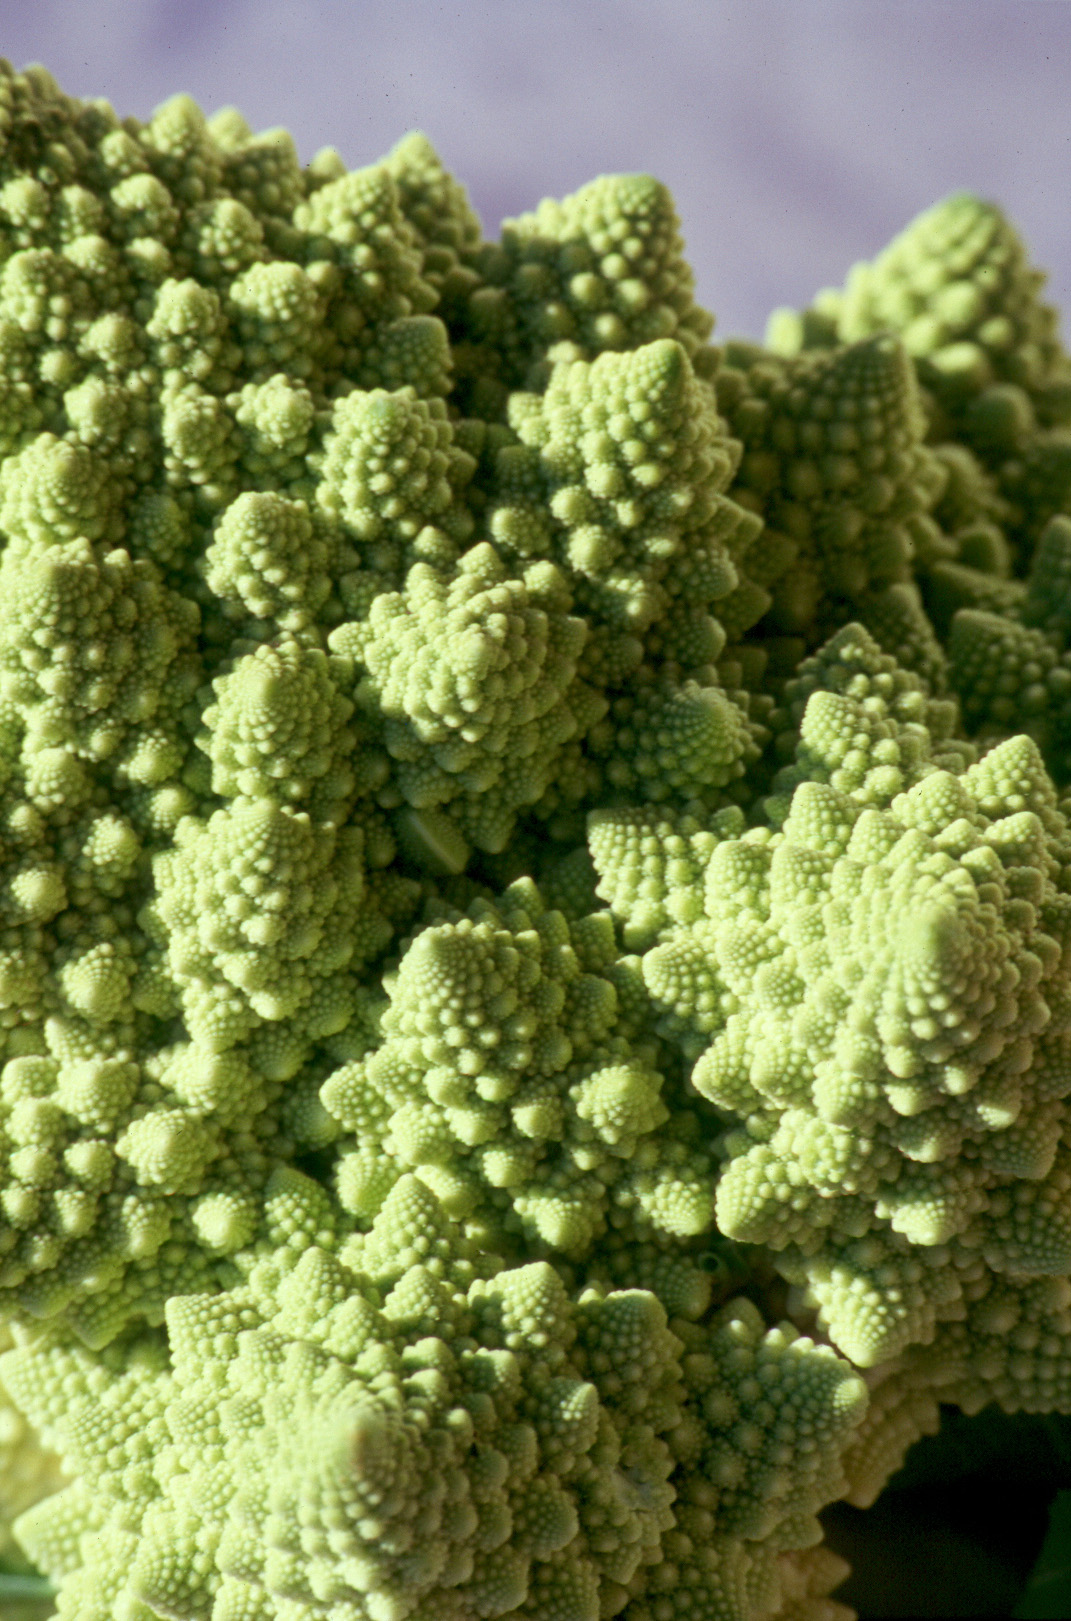
\includegraphics[width=.4\linewidth]{figures/Romanesco}
	\caption{Romanesco. Ein natürliches Fraktal. \cite{fractal_romanesco}}
	\label{fig:frac_kunst}
\end{subfigure}%
\begin{subfigure}{.5\textwidth}
	\centering
	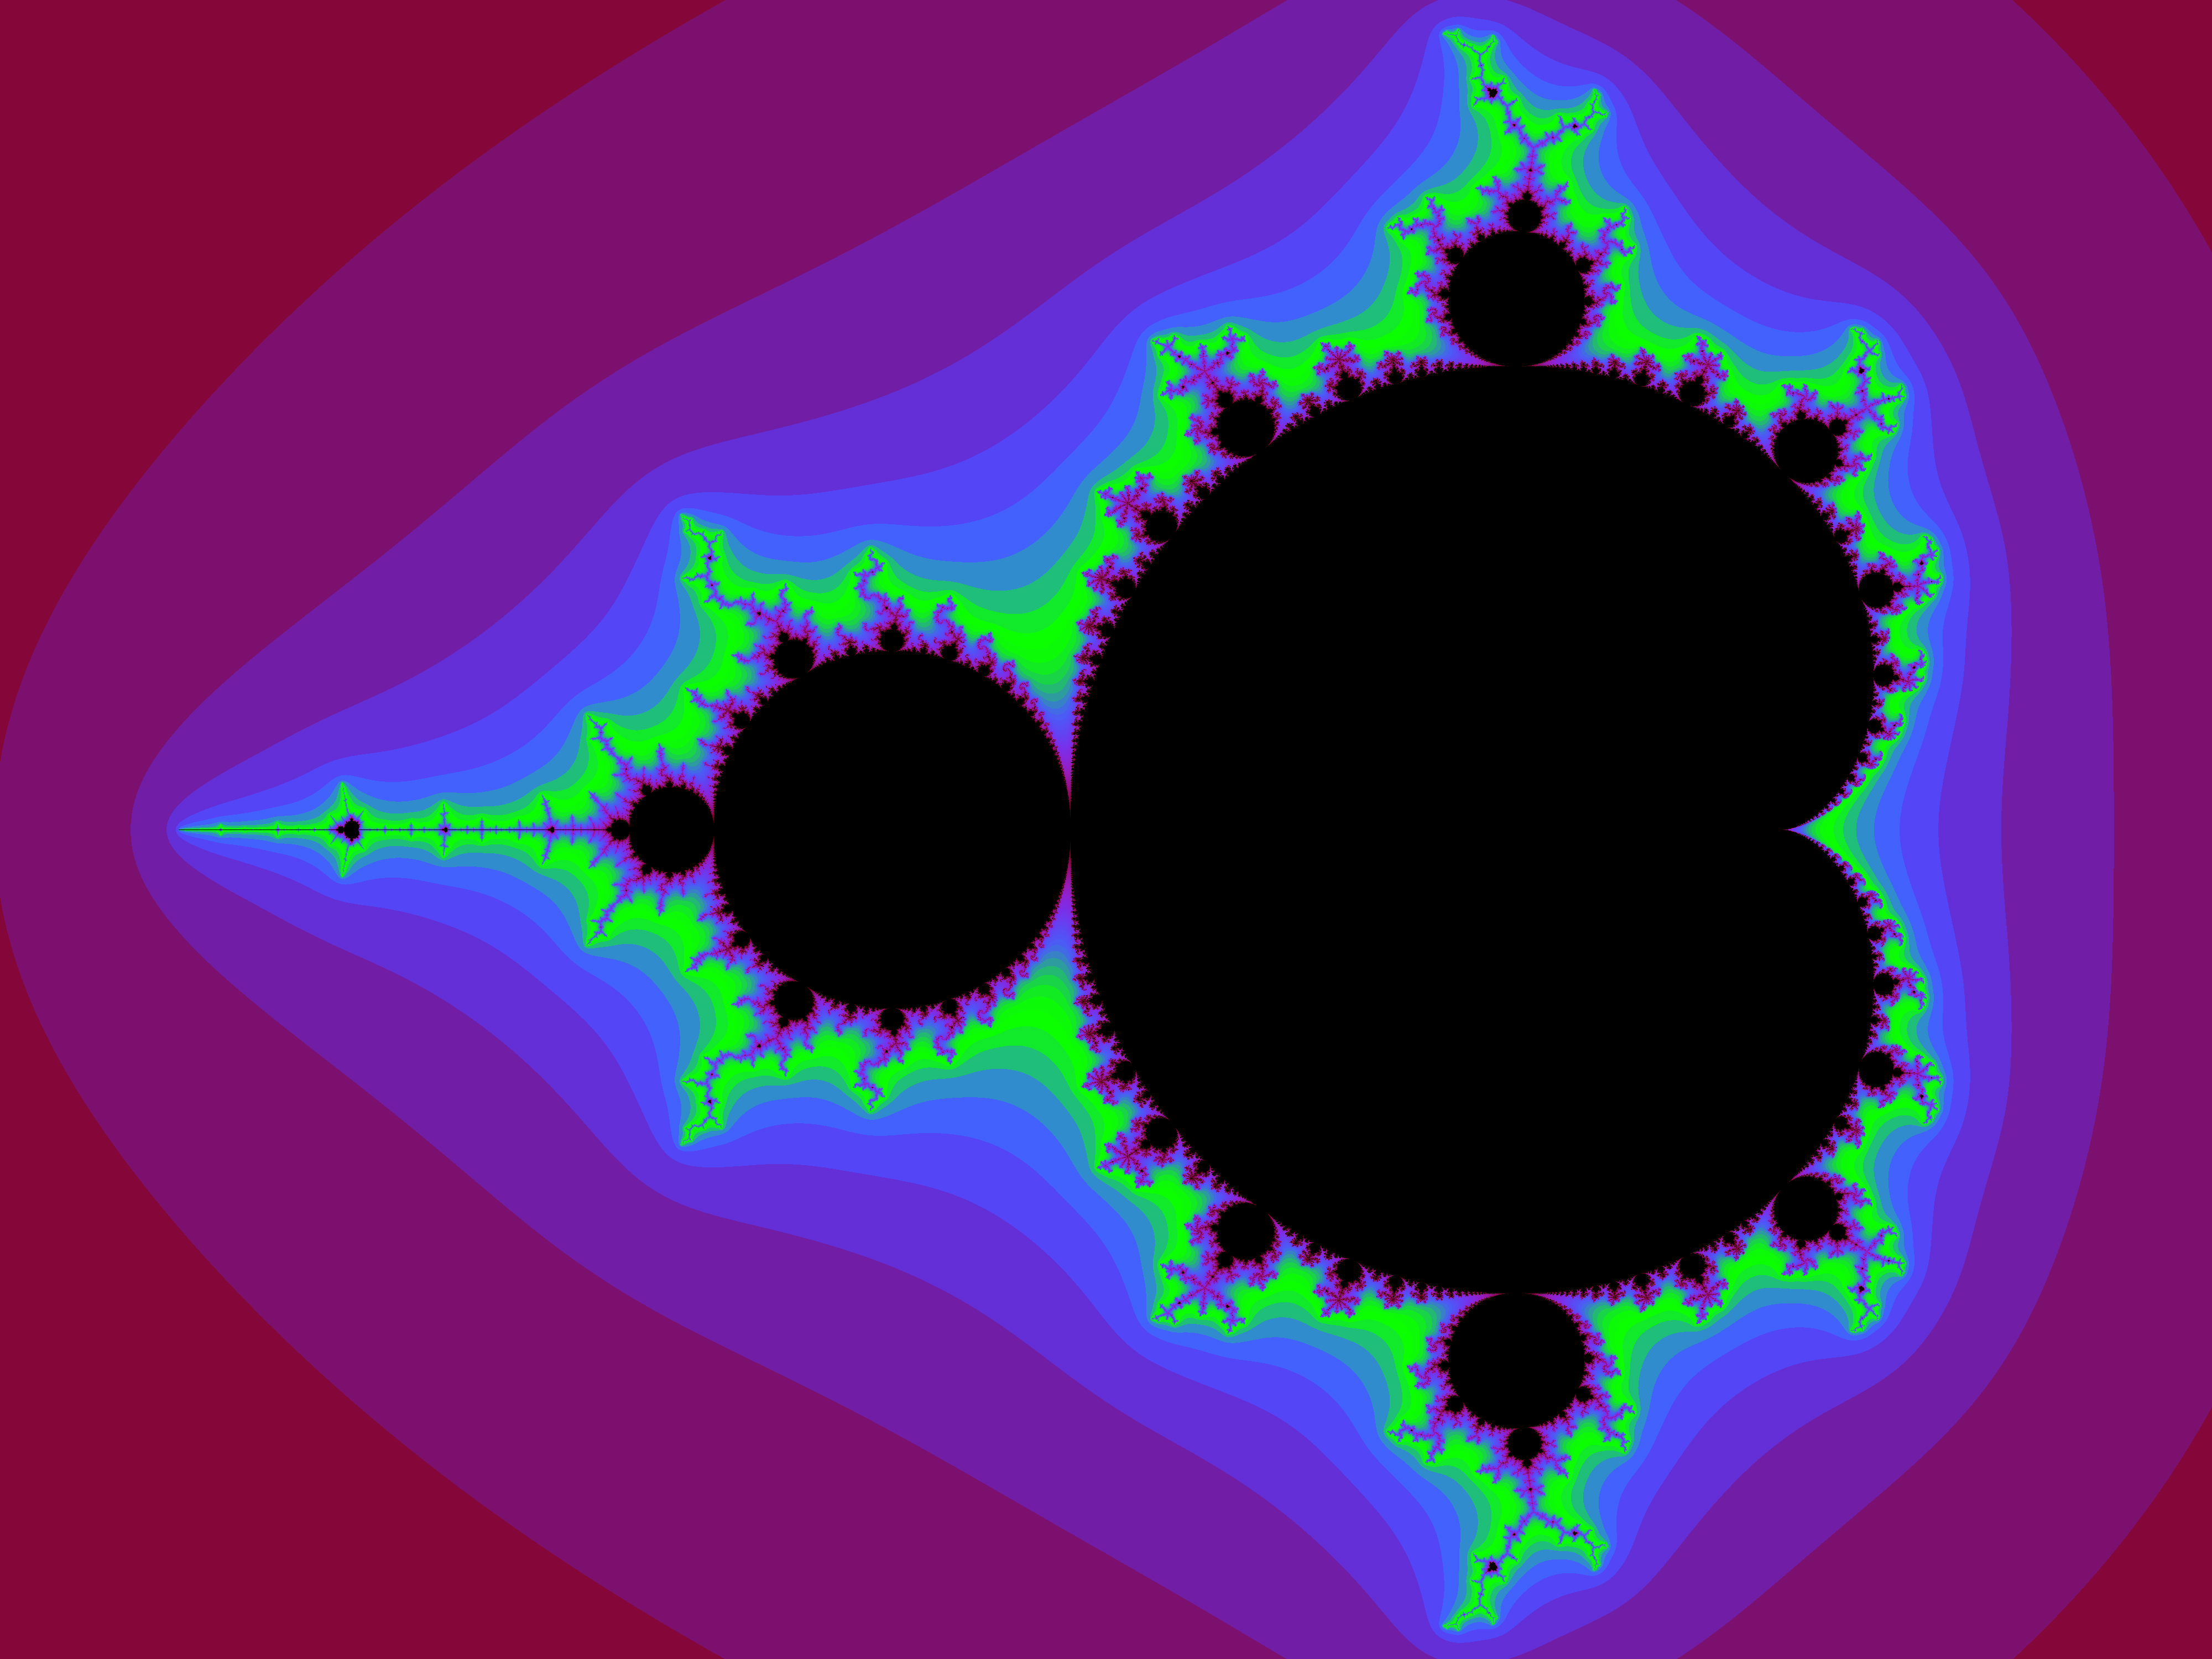
\includegraphics[width=.4\linewidth]{figures/Mandelbrot}
	\caption{Mandelbrot. Ein künstliches Fraktal. \cite{fractal_mandelbrot}}
	\label{fig:frac_math}
\end{subfigure}%
\end{figure}
\subsection{Newton Fraktale}
Diese Fraktale erscheinen sich, wenn man das Newton Verfahren für Auffinden der Wurzeln der nichtlinearen Gleichungen auf Komplexe Ebene benutzt.
Genauer gesagt, soll man die Wurzel für jeden Punkt des gesuchten Bildes mit Newton Verfahren finden.\\
Zum Beispiel nehmen wir die Funktion $f(x) = x^3 -1$. Diese Funktion hat drei Lösungen auf Komplexe Ebene: $1$, $-\sqrt[3]{-1}$ und $(-1)^{2/3}$. Näherungswerte in Koordinatenform sind $(1, 0)$, $(-0.5, 0.866)$ und $(-0.5, -0.866)$. Die Punkte des Bildes, die sich durch das Newton Verfahren zu entsprechenden Wurzeln annähern, werden entsprechend mit rot, blau und grün gefärbt.
Das Fraktal auf dem Bild \ref{fig:output3_0} repräsentiert die gewählte Umgebung.
Die Ursachen zu dieser komischen Mischung werden in der Sektion \ref{sec:analy} erläutert.
\begin{figure}[ht]   
	\centering
	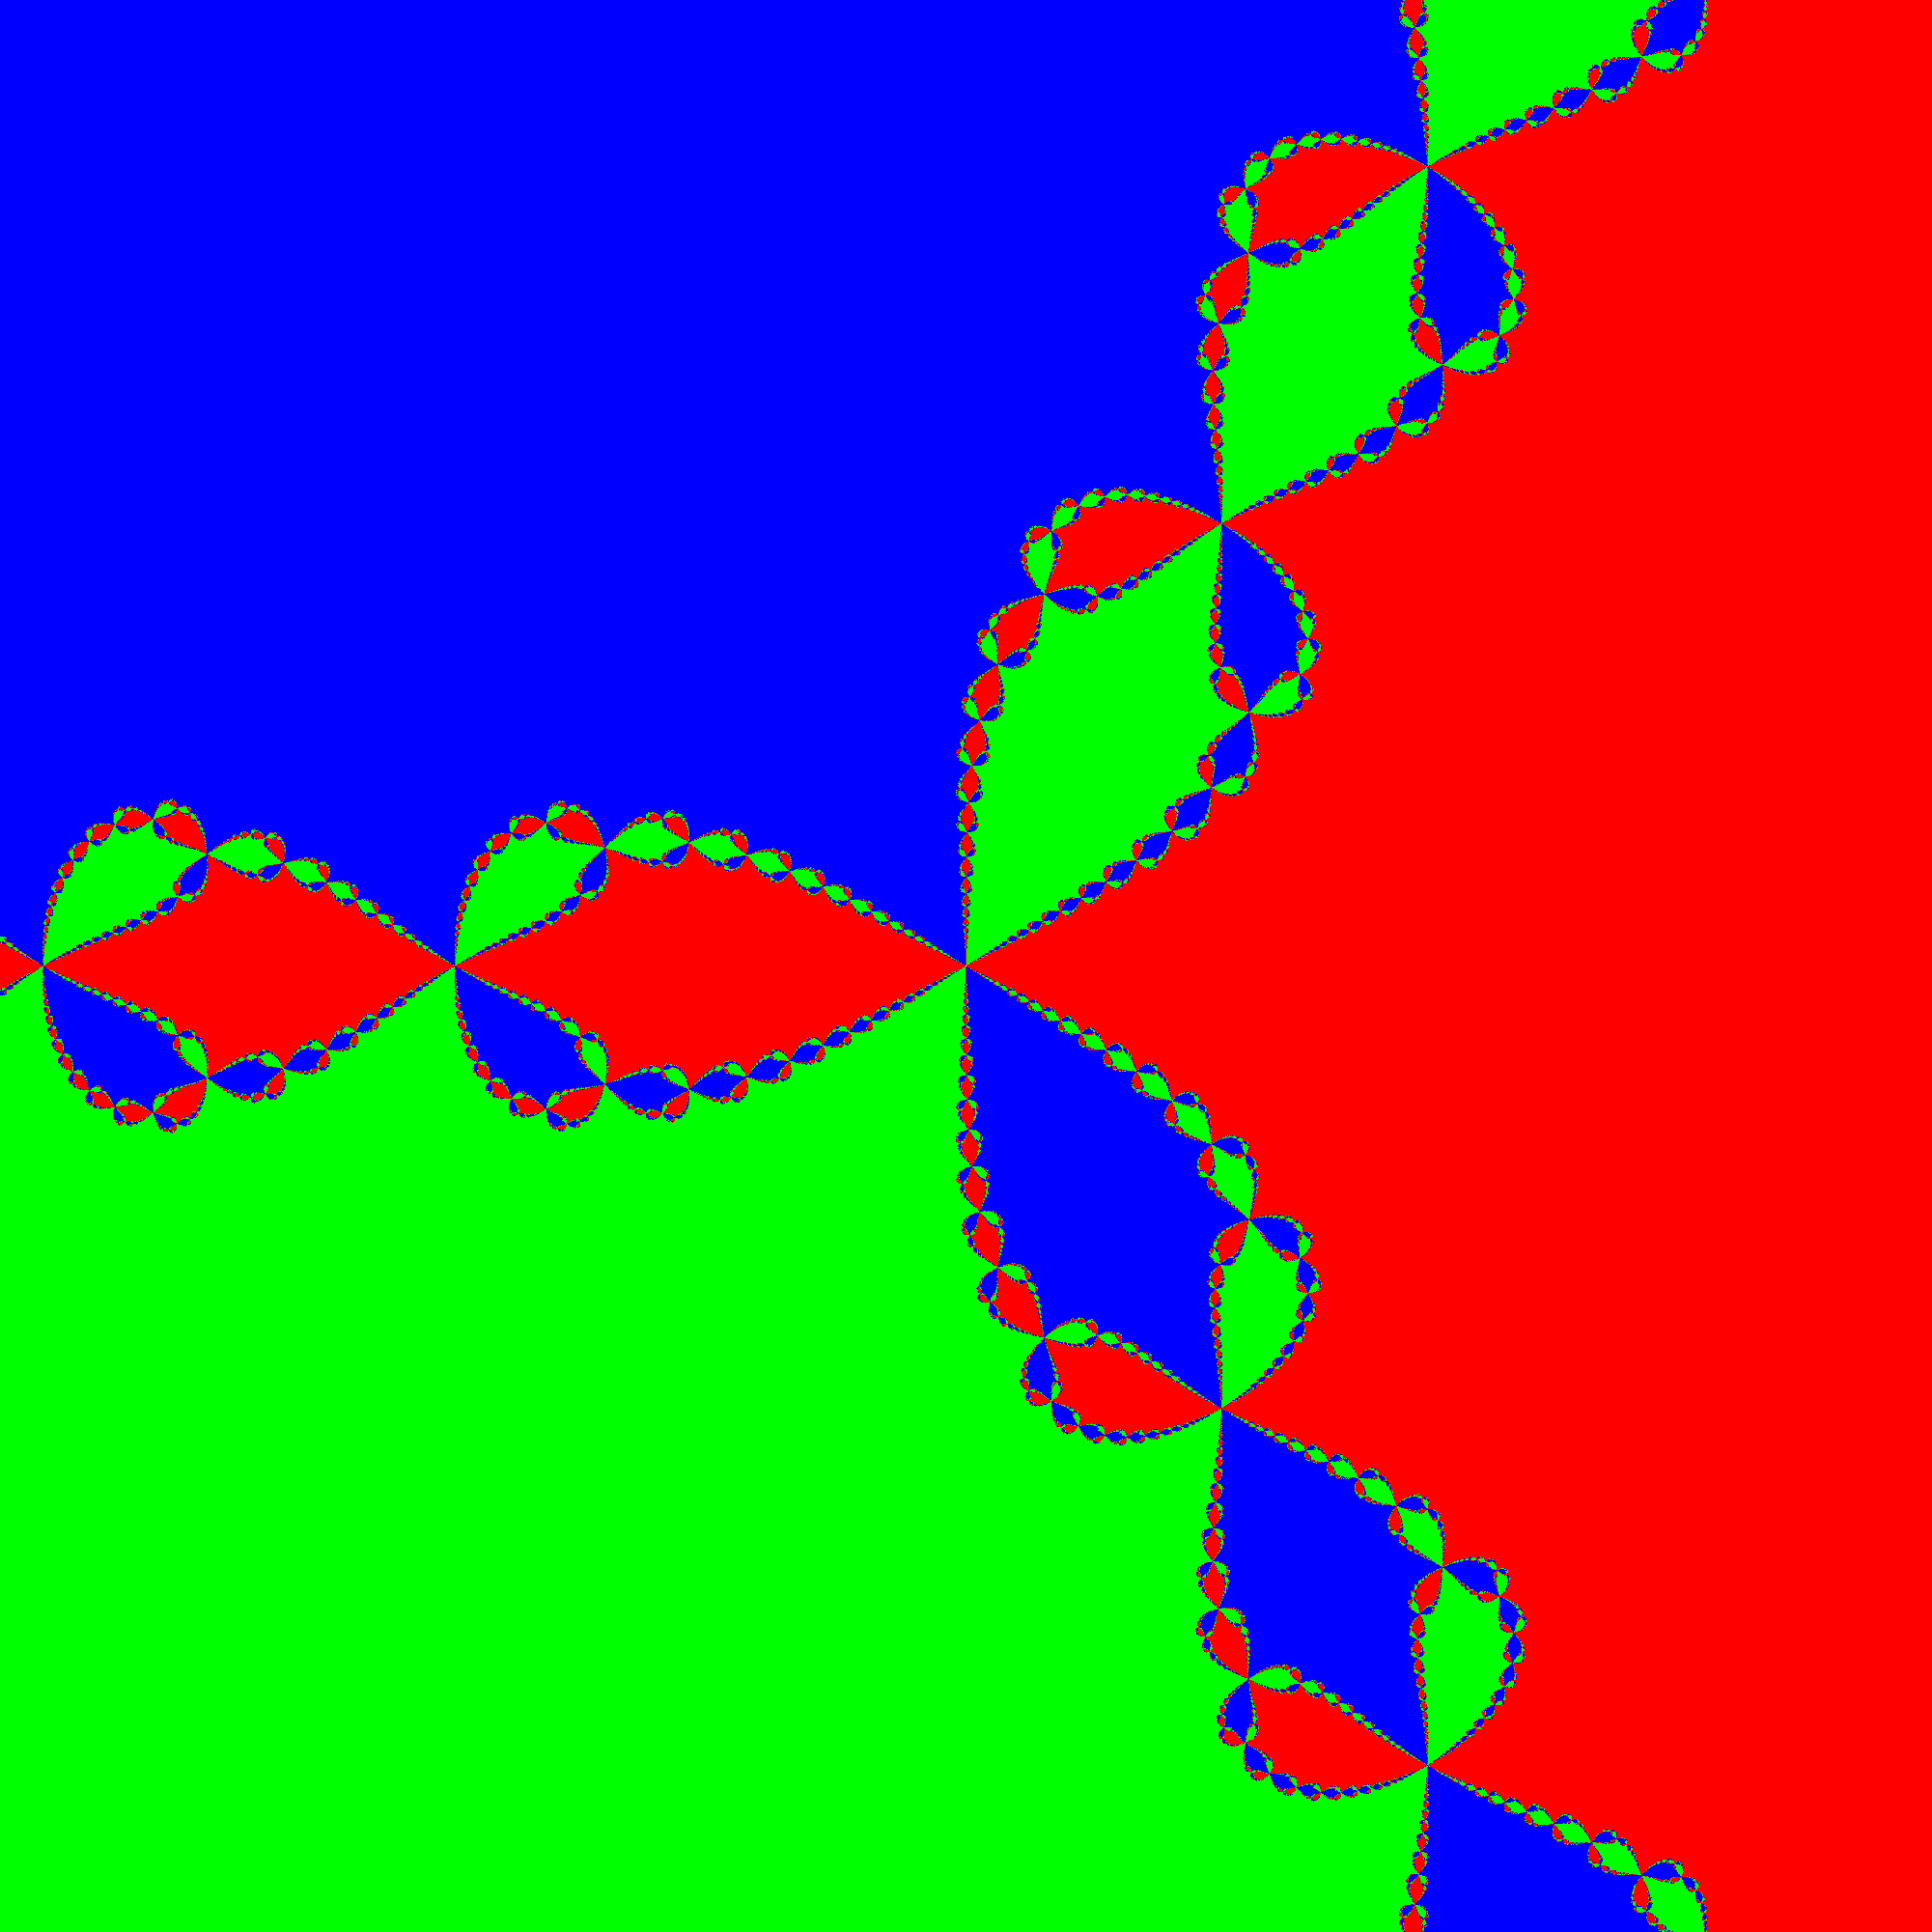
\includegraphics[width=.5\linewidth]{figures/output3_0}
	\caption{Newton Fraktal für $f(x)=x^3-1$ }
	\label{fig:output3_0}
\end{figure}
\section{Visualisierung}\label{sec:vis}
In diesem Abschnitt wird ein Programm entwickelt, das Bilder der Newton Fraktale generiert.
Außerdem es wird ein Beispiel vorgestellt, wie man Animationen erzeugen kann.
\subsection{Bildgenerierung}\label{subs:vis:bild}
Als Programmiersprache wurde Java gewählt.
\subsubsection{Bibliotheken}
Zusätzlich zu allgemeine Java-Bibliothek wurde noch das\\ $javax$.$imageio$.$ImageIO$ verwendet.
Das ist öffentliche Bibliothek für die Arbeit mit Bildern, das unter anderem für das .$png$ Format geeignet ist.
Das PNG (Portable Network Graphics) Format passt für unsere Ziele ideal, wegen kleines Gewicht und keinen Qualitätsverlust.
\subsubsection{Bild}
Mit Hilfe der $javax$.$imageio$.$ImageIO$ kann man sehr einfach die .$png$ Dateien erzeugen. Ein Beispiel in der Auflistung \ref{lst:png}.
\begin{lstlisting}[caption=Ein Beispiel für PNG Generierung, label=lst:png]
BufferedImage bi = new BufferedImage(w, h, TYPE_INT_ARGB) ;
ImageIO.write(bi, "png", outputfilename);
\end{lstlisting}
Um den Bildinhalt zu generieren, benutzen wir den $bi.setRGB(X, Z, Color);$ Befehl.\\
Natürlich soll man bestimmten Bereich wählen, um dann zu zeichnen. 
Bei unseres Programm wählt man den Startpunkt durch $X$ und $Y$ Koordinatenwerte, die Bildschirmgröße: $Size$ und die Auflösung: $resolution$. 
\subsubsection{Komplexe Zahlen}
Für die Bearbeitung der komplexen Zahlen wurden die entsprechende Klasse implementiert, die die Arbeit mit komplexen Zahlen erleichtert. 
Man kann komplexe Zahlen addieren, abrechnen, multiplizieren, dividieren und potenzieren.
\subsubsection{Newton Verfahren}
Um Newton Verfahren zu benutzen, soll man manuell die Ableitung berechnen, die Newton iterative Funktion ausfinden und im Programmkode umwandeln.
Als Beispiel nehmen wir die Funktion $f(z) = z^3 - 2z + 2$.
Entspreche Ableitung hat die Form $f'(z) = 3z^2 - 2$ und die iterative Funktion $z_{n+1} = \frac{2z_n^3 - 2}{3z_n^2 - 2}$.
Und hier steht der Programmkode für diese iterative Funktion.
\[
	devide(mult(hoch(wert,3),2).add(-2), mult(hoch(wert,2),3).add(-2));
\]
Natürlich nach jedem Schritt soll man Prüfen, ob die maximale Anzahl der Schritten $deep$ nicht überschreitet wird und ob der Punkt schon genug nah zu Nullstelle liegt. 
Das heißt, dass es für jeden gefundenen Punkt $z_n$ soll geprüft werden, ob $n > deep$ ist und $f|(z_n)| < toleranz$.
Falls einer der beiden Fälle eintritt, bricht man die iterative Berechnung ab.
Im ersten Fall bezeichnet man das Punkt mit weiße Farbe, im zweiten - mit Farbe assoziierte mit gefundener Lösung. 
\subsubsection{Lösungen} 
Da man manuell Farben für unterschiedliche Lösungen wählen will, war es entschieden, alle Lösungen mit assoziierten Farben im Programmkode eintragen. 
Ein Beispiel für die Funktion $z^3 - 1$ findet man in der Auflistung \ref{lst:punkt}
\begin{lstlisting}[caption=Lösungen mit Farben für $z^3 - 1$, label=lst:punkt]
points.add(new point(1,	   0,	   255, 0,   0));
points.add(new point(-0.5, 0.866,  0,   255, 0));
points.add(new point(-0.5, -0.866, 0,   0,   255));
\end{lstlisting}
\subsubsection{Schatten}
Für bessere Informationswiedergabe kann man die Schatten einschalten.
Dann je mehr Schritten des Newtonverfahren nötig sind, desto dunkler das Pixel wird.  
\subsubsection{Programmkode}
Vollständige Programmkode kann man unter \cite{source} finden.
\subsection{Animation}\label{subs:vis:anime}
Einer der einfachsten Wegen für die Animationserzeugung wurde gewählt. 
Das Programm wurde so geändert, dass $size$ und $outputfilename$ variabel werden. 
Dann im Zyklus wird eine Reihenfolge der Bildern generiert, so dass neues Bild die Annäherung des Alten wird.
Dann aus diese Reihenfolge mit Hilfe des \cite{animegen} wurde die Animation generiert.
\section{Analyse}\label{sec:analy}
Es werden manche Newton Fraktale vorgestellt und analysiert.
\subsection{$z^3 - 1 = 0$}
Wie oben schon gesagt war, hat diese Gleichung drei Lösungen auf Komplexe Ebene: $+1$, $-\sqrt[3]{-1}$ und $(-1)^{2/3}$ und war auf dem Bild \ref{fig:output3_0} visualisiert. 
Wenn man versucht die Grenze zwischen zwei Zonen zu annähern, sieht man, dass dort immer dritte Zone vorkommt. 
Das wiederholt sich rekursiv bei Annäherung.
In anderen Worten, wenn man einen Anfangspunkts $z_0$ wählt, der gegen $+1$ konvergiert und einen Punkt $z_1$, der gegen  $-\sqrt[3]{-1}$ konvergiert, dann existiert es immer einen dritten Punkt $z_2$, der noch näher zu $z_0$ als $z_1$ liegt und zu $(-1)^{2/3}$ konvergiert. \\
Wichtigste Frage ist: warum sehen die Zonen nicht wie die einfachen 120-Grad-Sektoren aus?
Anfang letztes Jahrhunderts gelang es zwei französischen Mathematiker Gaston Julia und Pierre Fatou zu zeigen, dass die Grenzpunkten eines Einzugsgebiets die Grenzpunkte aller Einzugsgebiete sind. 
Folglich können Iterationen mit mehr als zwei Einzugsgebieten keine einfach zusammenhängenden Liniensegmente als Gebietsgrenzen in 2D haben. 
Solche Grenzen müssen zwangsläufig fraktalen Natur sein, bestehend aus vollständig separaten Punktmengen - sozusagen eine unendlich feine Staubwolke aus nichtabzählbar vielen Staubpartikelchen.~\cite{frak_cha}
Machen wir uns damit ein bisschen vertraut, indem wir die Nullstelle (der Punkt $0:0$) anschauen.
Logischerweise soll die Nullstelle zwischen allen Zonen liegen und Null selbst konvergiert überhaupt nicht, da bei Newton Verfahren für diese Funktion, $z=0$ zu Division durch Null folgt.
Aber diese Nullstelle ist nicht allein, außerdem existieren noch unendlich viele Punkte, die gegen die Null konvergieren und für die auch gilt, dass daneben sich alle Zonen befinden.
(Das folgt aus die lineare Natur des Newton Verfahrens.)
Diese Punkten, die gegen die Null konvergieren, bilden diese komische Grenze Zwischen Zonen. 
Zum Beispiel betrachten wir ein paar Punkte. 
Konvergenz des Punktes (1, 1) wird auf dem Bild \ref{fig:output_points3} vorgestellt.
\begin{figure}[ht]   
	\centering
	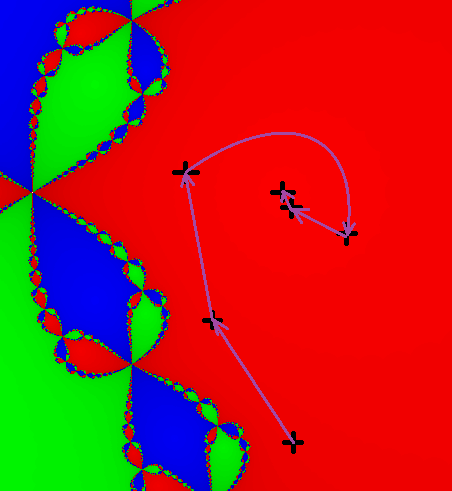
\includegraphics[width=.5\linewidth]{figures/output_points3}
	\caption{Konvergenz des Punktes (1, 1) für $f(x)=x^3-1$ }
	\label{fig:output_points3}
\end{figure}
Der Punkt liegt weit genug von der Grenze und wird eindeutig konvergiert, trotzdem sieht man so ein Sprung, die sehr oft bei Newton Verfahren eintreten werden.\\
Jetzt betrachten das Punkt (0.9, 1) auf dem Bild \ref{fig:output_points_g3}.
  \begin{figure}[ht]   
  	\centering
  	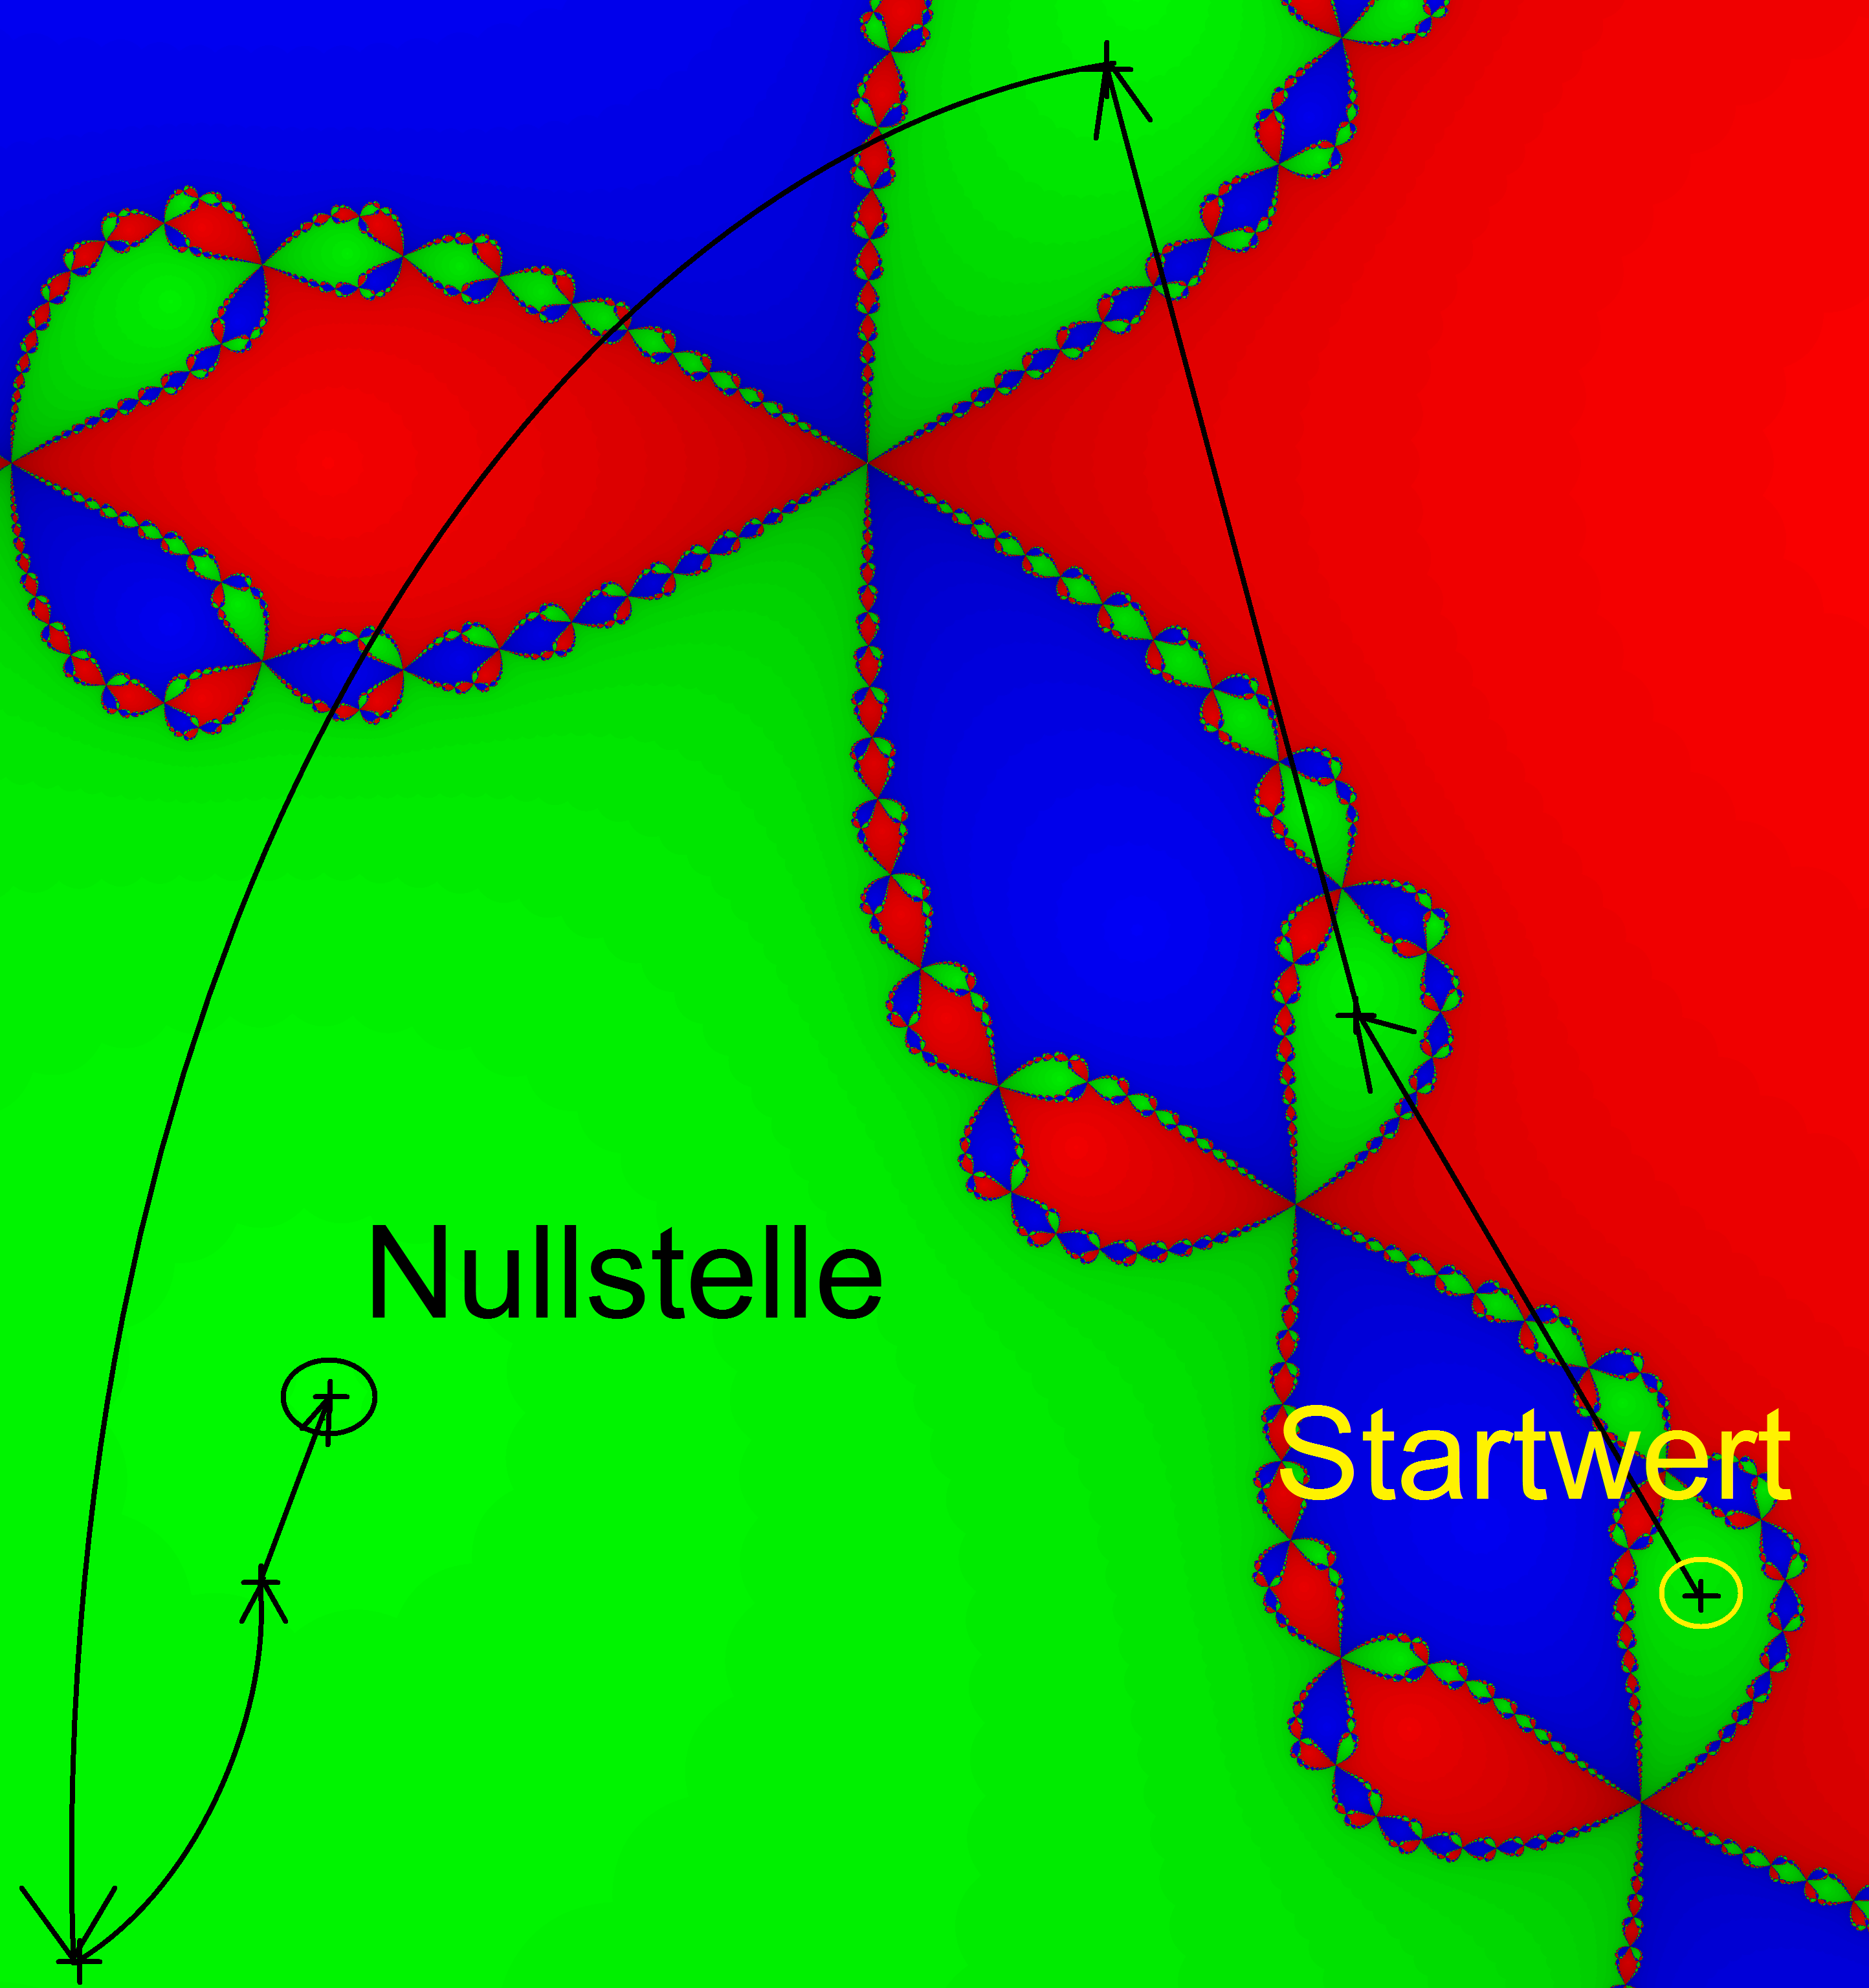
\includegraphics[width=.5\linewidth]{figures/output_points_g3}
  	\caption{Die Konvergenz des Punktes (0.9, 1) für $f(x)=x^3-1$ }
  	\label{fig:output_points_g3}
  \end{figure}
Die Konvergenz des Punktes zeigt eindeutig, wie die iterative Schritte des Newton Verfahrens funktionieren und wie man zu solchen Bildern kommt. 
Erste drei Punkte sind gleich zu die Konvergenz des Punktes (1, 1), was die lineare Natur des Newton Verfahrens bekräftigt, aber dann, neben der Nullstelle, wird die Konvergenz nach grünen Gebiet geworfen.
Die Punkten neben Grenzen bewegen sich zuerst in die Richtung der Nullstelle und dann rasant in die passende Zone springen.\\
Zusätzliches Beispiel wird auf Bild \ref{fig:output3_3} vorgestellt, wo helle Bereiche am schnellsten zu Lösungen konvergierende Punkte bezeichnen.
\begin{figure}[ht]   
	\centering
	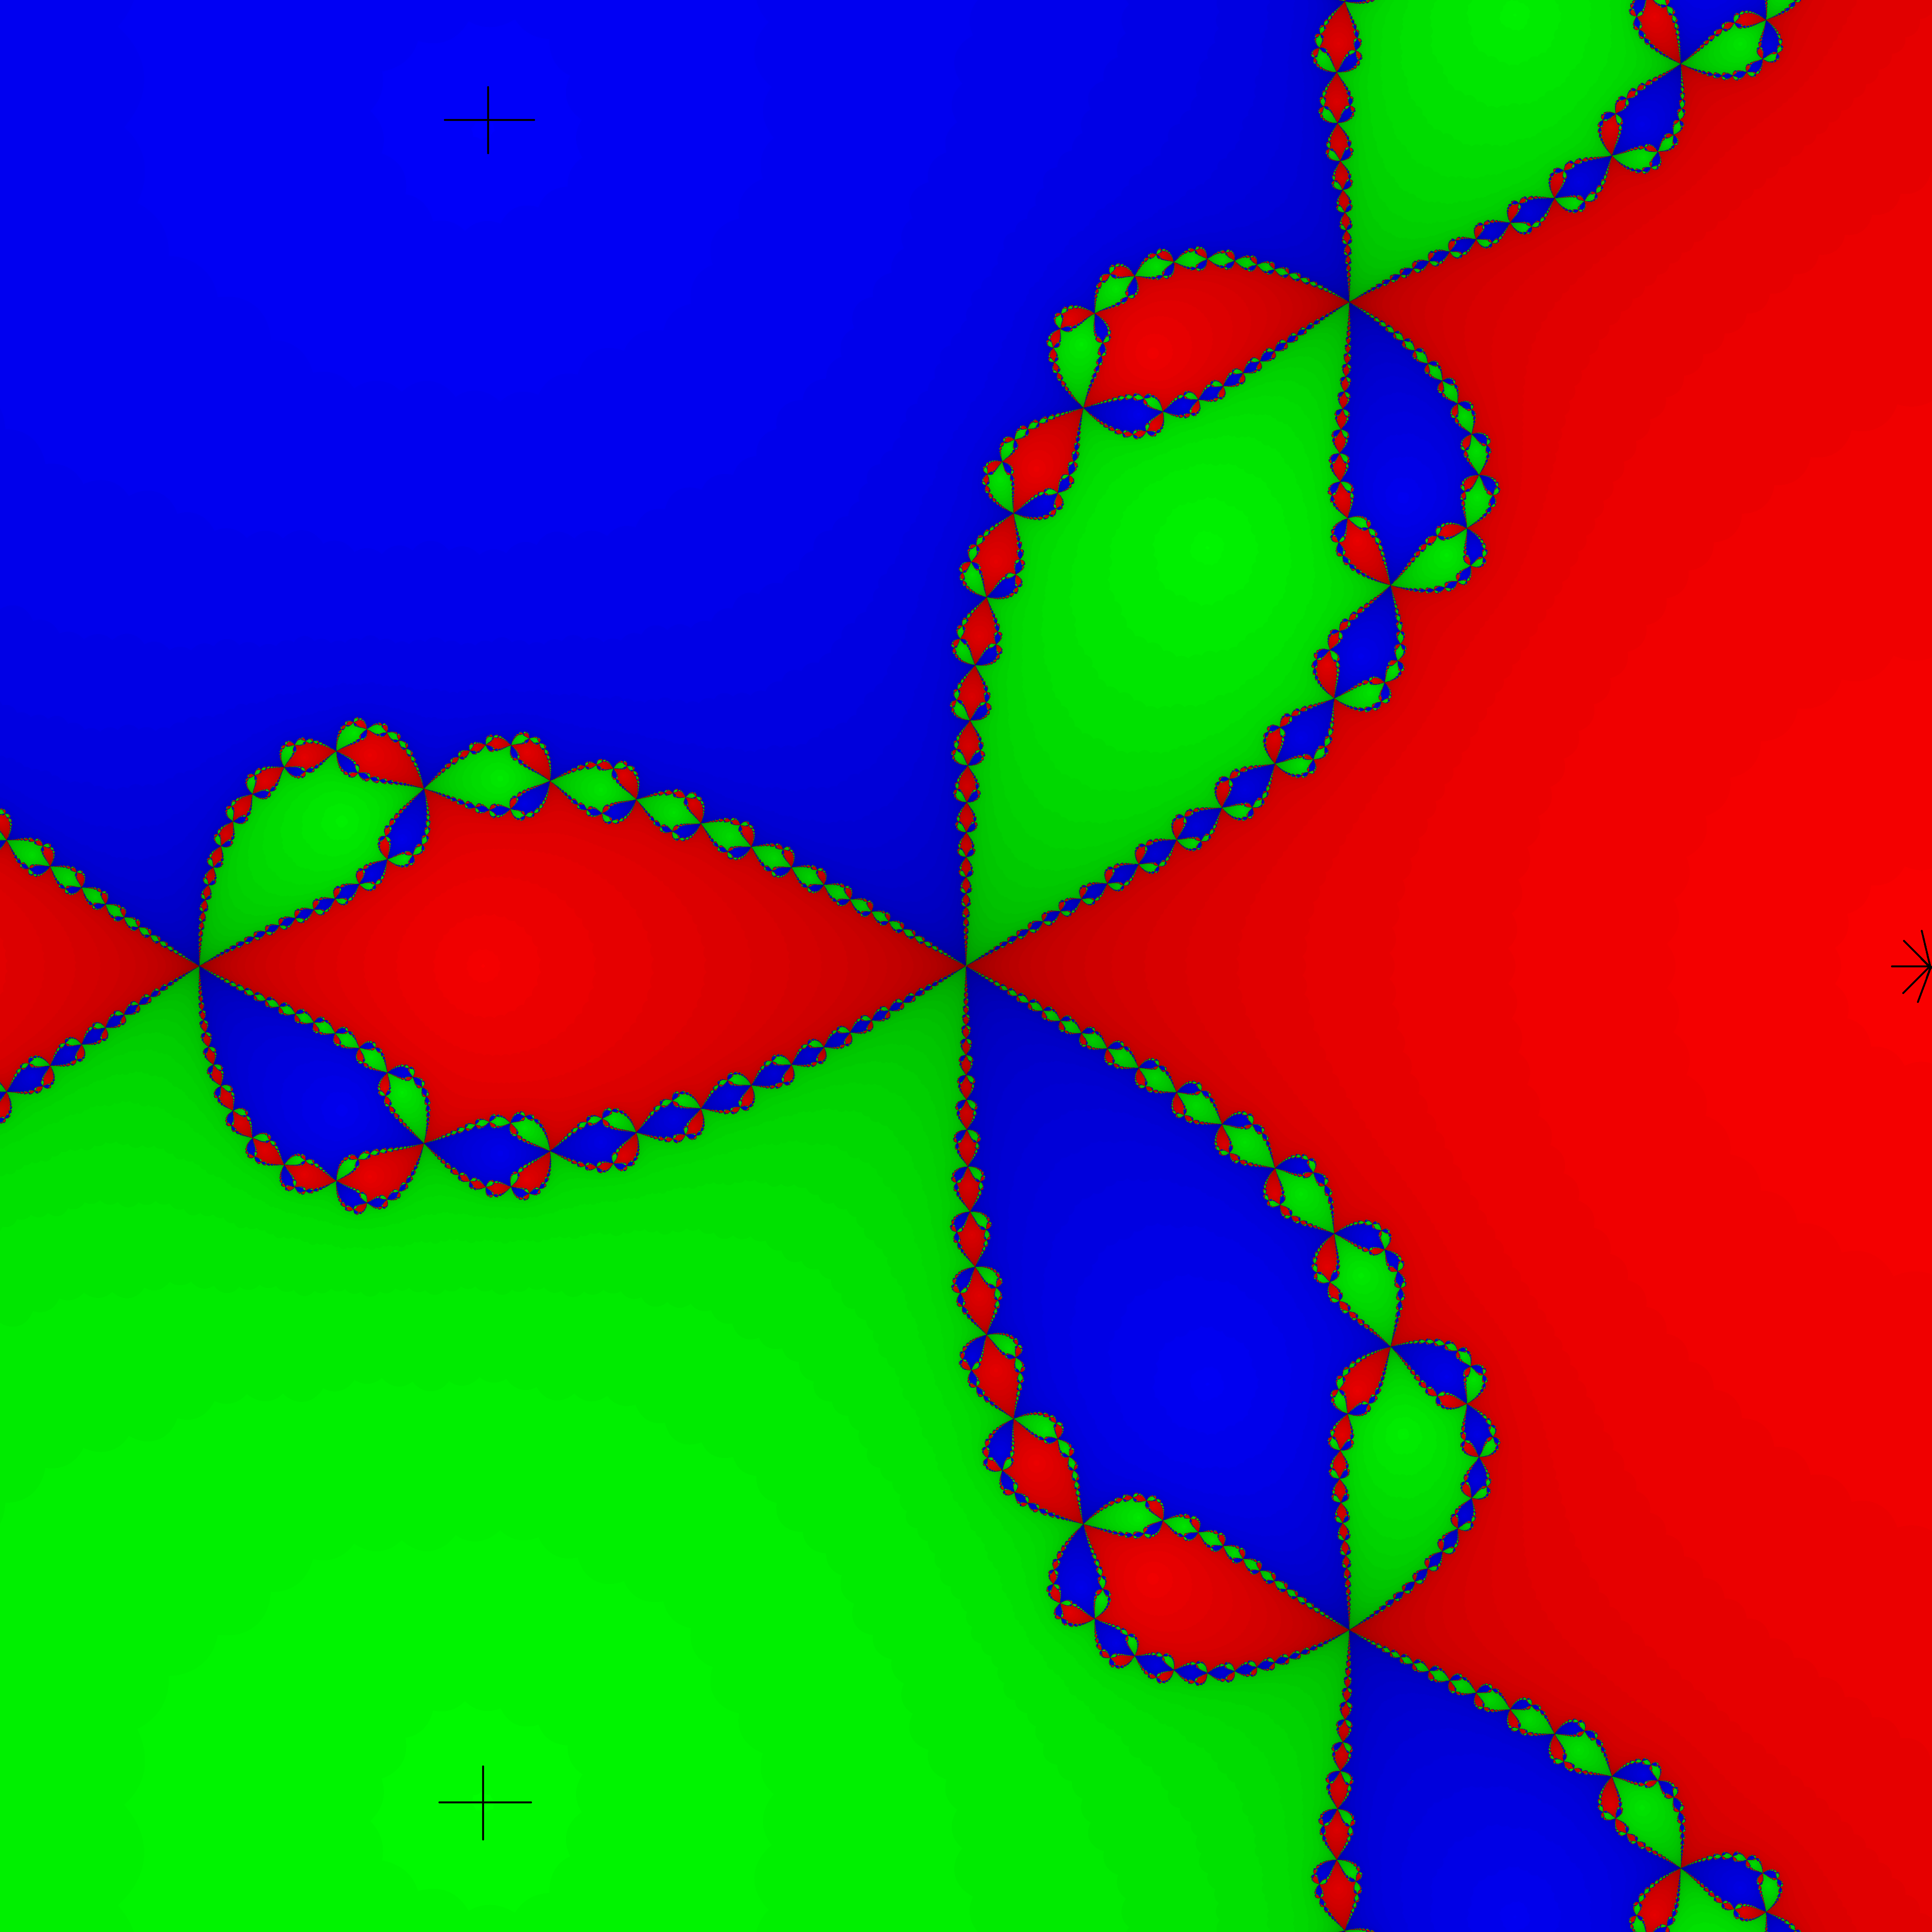
\includegraphics[width=.5\linewidth]{figures/output3_3}
	\caption{Die Konvergenzgeschwindigkeit durch die Helligkeit für $f(x)=x^3-1$ }
	\label{fig:output3_3}
\end{figure}

\subsection{$z^5 -1 = 0$}
Das Bild \ref{fig:output5_3} illustriert das Newton Fraktal. 
Einziegen Unterschied liegt in der Anzahl der Zonen und Lösungen: hier gibt es 5 beides.
Wie bei $z^3 -1 = 0$ sind die Grenzpunkten eines Einzugsgebiets die Grenzpunkte aller Einzugsgebiete.
\begin{figure}[ht]   
	\centering
	\includegraphics[width=.5\linewidth]{figures/output5_3}
	\caption{Das Newton Fraktal für $f(x)=x^3-1$ }
	\label{fig:output5_3}
\end{figure}
\section{Zusammenfassung}
\if 0

\fi
% Literaturverzeichnis ------------------------------------------------
\newpage
\bibliographystyle{alphadinLinkLocal}
\bibliography{literatur} 

%\iffalse
\end{document}
%\fi
